\usetikzlibrary{arrows}
\renewcommand{\familydefault}{\sfdefault}
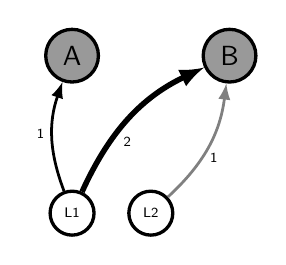
\begin{tikzpicture}[node distance=2cm, auto, thick, scale = 2.0, font=\tiny]
    \tikzstyle{node_black} = [draw=black, very thick, circle, fill=gray!80, shorten <=1pt, shorten >=1pt, font=\sf]
    \tikzstyle{node_empty} = [draw=black, very thick, circle, fill=none, font=\sf\tiny]
    \tikzstyle{arrow_black} = [->, black, >=latex]
    \tikzstyle{arrow_grey} = [->, gray, >=latex]

    \node[node_black] (nA) at (0,1) {A};
    \node[node_black] (nB) at (1,1) {B};
    \node[node_empty] (n0) at (0,0) {L1};
    \node[node_empty] (n1) at (0.5,0) {L2};

    \draw[arrow_black, line width=1] (n0) edge [bend left=20] (nA);
    \draw[arrow_black, line width=2] (n0) edge [bend left=20] (nB);
    %\draw[arrow_grey, line width=1] (n1) edge [bend right=20] (nA);
    \draw[arrow_grey, line width=1] (n1) edge [bend right=20] (nB);

    \node[draw=none] at (-0.2,0.5) {1};
    \node[draw=none] at (0.35,0.45) {2};
    \node[draw=none] at (0.90,0.35) {1};

\end{tikzpicture}
